\documentclass[12pt]{article}
\usepackage[utf8]{inputenc}
\usepackage[spanish]{babel}
\usepackage{enumerate}
\usepackage{graphicx}
\usepackage{listings}
\usepackage{graphicx}
\usepackage[hidelinks]{hyperref}
\usepackage[vmargin=3cm,hmargin=2cm]{geometry}

\title{\textbf{\underline{CLIPS:}\\
		 Sistema Experto para asesorar a un	inversor en bolsa.}}
\author{\textbf{ Autora:} Cristina Zuheros Montes - 50616450\\
	    \href{https://github.com/cristinazuhe}{Enlace a Github}}
\date{\textbf{Fecha:} 30 Junio 2016}
\begin{document}

\maketitle

\tableofcontents

\newpage
\section{Cómo funciona el Sistema Experto. }\label{PrimeraSeccion}
 Vamos a desarrollar un Sistema Experto en CLIPS que sea capaz de asesorar a un inversor con una cartera de acciones en valores del Ibex 35.\\
 
 Nuestro sistema dispondrá diariamente de la información de los valores de cierre del día anterior de las empresas del Ibex 35. Esta información estará almacenada en distintos archivos \textit{nombre\_archivoX.txt}.\\
 
 Además será capaz de leer la información sobre la cartera del usuario para conocer las inversiones actuales del mismo. Esta información sobre la cartera del usuario se la proporcionará al Sistema Experto el propio usuario mediante un archivo \textit{nombre\_cartera.txt}. En él se indicará el nombre de la empresa, el número de acciones del que dispone y la valoración actual de esas acciones, es decir, el valor económico que tienen en el momento. \\
 
 Asimismo el Sistema Experto va a solicitarle al usuario información sobre si ha habido noticias malas o buenas sobre las empresas del Ibex 35 en los últimos 3 días. Esta información se proporcionará a través de un archivo \textit{nombre\_noticias.txt}. En él se indicará el nombre de la empresa, si la noticia es buena o mala y el número de días que tiene la noticia de antigüedad. \\
 
 Una vez que nuestro Sistema Experto ya dispone de todo el conocimiento necesario, va a razonar como el experto lo haría y va a proponer al Usuario hasta las 5 mejores opciones de compra-venta de valores, indicando los motivos por lo que aconseja estas propuestas. \\
 
 Una vez que el usuario visualiza las opciones, tendrá la opción de aceptar alguna de estas sugerencias. En este caso, el sistema actualizará la información en cartera del usuario y propondrá nuestras propuestas en base a dicha actualización. 
 


 
\newpage
\section{Descripción del proceso seguido para el desarrollo. }
\subsection{Sesiones con el experto, indicando información obtenida en cada una de ellas.}
Para poder desarrollar nuestro Sistema Experto hemos tenido que realizar varias reuniones con el experto. 

\begin{center}
	\underline{\textbf{Primera sesión.}}
\end{center}

Hemos obtenido los objetivos básicos del sistema. Además hemos tratado de informarnos sobre qué datos necesita y de dónde los podremos extraer, para así poder tener toda la información a tratar en nuestro alcance. Le hemos realizado preguntas al experto como:\\

\textbf{- ¿Qué datos usará nuestro sistema?}\\
Básicamente usaremos datos sobre las empresas y sobre los sectores de dichas empresas del Ibex35. Además tendremos noticias sobre las empresas y sectores y contaremos con la cartera del usuario. \\

\textbf{- ¿De dónde obtenemos dichos datos?}\\
Los datos de empresas y sectores del Ibex 35 los obtendremos de la web de la bolsa de Madrid. La cartera y las noticias las proporciona el usuario. \\

\textbf{- ¿Cuántas sugerencias quieres que te muestre el sistema?}\\
Quiero las 5 mejores propuestas. \\

\begin{center}
	\underline{\textbf{Segunda sesión.}}
\end{center}

Nos hemos preocupado por conocer qué significa para el usuario que un valor sea peligroso. Nos centremos en la pregunta "¿Bajo qué conceptos vamos a definir si un valor es o no peligroso?". Aquí nos surgen preguntas sobre:\\

\textbf{- ¿Cuándo un valor es inestable?}\\
Bien cuando la empresa sea del sector de la construcción o bien cuando la economía esté bajando y la empresa sea del sector servicios o bien cuando haya ciertas noticias malas sobre la empresa, su sector o el Ibex. \\

\textbf{- ¿Que quiere decir que la economía esté bajando?}\\
Que el valor en los últimos 3 días esté bajando. Con valor nos referimos a la media de los valores del Ibex35. \\

\textbf{- ¿Cuándo un valor es estable?}\\
Un valor pasa a ser estable si alguna noticias positivas sobre la empresa o su sector.

\textbf{- ¿Qué hacer cuándo tenemos noticias negativas y positivas que impliquen a una misma empresa?}\\
La información más específica es la que predonima. \\

\begin{center}
	\underline{\textbf{Tercera sesión.}}
\end{center}

Con el experto obtenemos información sobre qué significa para él que un valor este infravalorado o sobrevalorado. Realizamos preguntas como:\\

\textbf{- ¿Cuándo podemos decir que una empresa ha caido bastante en X tiempo?}\\
Que su variación en X tiempo haya caido más del 30\%.\\

\textbf{- ¿Cuándo podemos decir que una empresa ha subido, pero no mucho en el mes?}\\
Que la variación del mes sea positiva pero inferior al 10\%.

\textbf{- ¿Qué quiere decir que una empresa se comporte mejor o peor que su sector?}\\
Que la variación de la empresa sea mejor o peor que la de su sector. 

\bigskip
\bigskip
\bigskip
\bigskip
\subsection{Procedimiento de validación y verificación del sistema seguido.}
Hemos probado el sistema para comprobar que, efectivamente, cumple su funcionamiento requerido.\\
Algunos aspectos que hemos tratado para que todo funciones correctamente o que se han prestado a confusión y se merecen una mención destacada son:\\

\begin{center}
	\textbf{¿Comprar acciones o invertir dinero?}
\end{center}
Este es un punto importante que puede prestar a confusión con las peticiones que se han solicitado al sistema. Si nuestro Sistema Experto propone que se invierta en una empresa, podríamos pensar en comprar X acciones o bien en invertir X dinero para comprar tantas acciones como se pueda. \\

Si el usuario indica la cantidad de dinero que quiere comprar, seguramente indicará una cantidad de dinero no proporcional a la cantidad entera de acciones que puede comprar de la empresa. Por este motivo, hemos considerado que es mejor solicitar el número de acciones que quiere comprar y comprarlas si de verdad el usuario tiene dinero disponible. \\

Es un aspecto que puede modificarse fácilmente pero, como el experto no lo ha especificado, hemos optado por la opción indicada anteriormente por la propia comodidad del usuario. \\

\begin{center}
	\textbf{Permitir comprar acciones.}
\end{center}
Cuando vamos a cambiar ciertas acciones de una empresa de la cartera a otra, esté o no en la cartera, vamos a tener que comprobar que si las acciones de la primera empresa cuestan menos que las acciones de la segunda empresa, tengamos dinero suficiente disponible para el desfase que se produce de dinero.\\

Vamos a optar por hacer el cambio de las acciones de una empresa a otra siempre y cuando el usuario tenga dinero disponible suficiente. De modo que el usuario tiene que ser consciente de que el cambio le puede suponer dicho coste.\\

\begin{center}
	\textbf{Cotización de las empresas.}
\end{center}
El precio de las acciones depende de la empresa en cuestión. Este precio lo tendremos indicado en el archivo de las empresas en la variable Precio. Pero además, si tenemos compradas acciones de la empresa, lo podremos calcular a partir de los valores de la cartera del usuario, pues en ella disponemos de la cantidad de acciones que tenemos y del precio que tienen todas estas acciones en el momento.\\

Para realizar algunos razonamientos en nuestro Sistema Experto, hemos utilizado la cotización de la empresa mirándola en el archivo de las empresas o mirando los datos de la empresa que tenemos en cartera, según nos ha ido interesando para que en ningún momento tengamos resultados extraños por décimas que puedan variar. \\

Hemos ido comprobando con distintas situaciones que todo se haga correctamente.\\ 



\newpage
\section{Descripción del sistema desarrollado.}
\subsection{Variables de entrada del problema}
Ya hemos comentado que nuestro sistema va a ser uno de distintas variables de entrada:

\begin{center}
	\textbf{Datos básicos de las empresas.}
\end{center}
Lo primero que hacemos en nuestro sistema, va a ser cargar los datos sobre las empresas. Para ello vamos a definir un deftemplate que contenga tantos slot como variables de cada empresa. La estructura quedaría del siguiente modo:

\begin{lstlisting}
(deftemplate Empresas
	(slot Nombre)
	(slot Precio)
	(slot VariacionDia)
	(slot Capitalizacion)
	(slot PER)
	(slot RPD)
	(slot Tamanio)
	(slot PorcentIBEX)
	(slot EtiquetaPER)
	(slot EtiquetaRPD)
	(slot Sector)
	(slot Var5Dias)
	(slot Perd3Dias)
	(slot Perd5Dias)
	(slot VarSector5Dias)
	(slot VRS5)
	(slot VarMes)
	(slot VarTrimestre)
	(slot VarSemestre)
	(slot VarAnual)
)
\end{lstlisting}


Para cargar estos datos de las empresas, vamos a crear un fichero auxiliar al que llamaremos \textit{LecturaEmpresa.CLP}.

Vamos a explicar brevemente lo que hacemos en este archivo ya que lo hacemos para leer los distintos datos que necesita nuestro sistema:

En primer lugar creamos una regla que nos permita abrir el archivo. A continuación, leemos los datos del fichero mediante (read file) y situamos cada variable de la empresa en su correspondiente slot. Finalmente, tenemos otra regla con la que cerramos el archivo. Nos hemos basado en el esquema del pdf proporcionado llamado \textit{"Ejemplo Leer datos de un fichero procesarlos y guardarlos (CLIPS).pdf"}.

De este modo, ya tenemos los datos de las empresas disponibles para usarlos en nuestro Sistema Experto. 

\begin{center}
	\textbf{Datos básicos de los sectores.}
\end{center}
Una vez que tenemos cargados los datos de la empresas, vamos a cargar los datos de los sectores a los que pueden pertenecer las empresas. Definimos otra estructura deftemplate con tantos slot como variables tienen los sectores. La estructura quedaría del siguiente modo:
\begin{lstlisting}
(deftemplate Sector
	(slot Nombre)
	(slot VariacionDia)
	(slot Capitalizacion)
	(slot PERMedio)
	(slot RPDMedio)
	(slot PorcentIBEX)
	(slot Var5Dias)
	(slot Perd3Dias)
	(slot Perd5Dias)
	(slot VarMes)	
	(slot VarTrimestre)
	(slot VarSemestre)
	(slot VarAnual)
)
\end{lstlisting}
De nuevo, creamos un fichero auxiliar \textit{LecturaSectores.CLP} que nos va a permitir obtener los datos de los sectores y almacenarlos en la estructura que acabamos de ver. El código es similar al comentado para las empresas. \\
Finalmente merece la pena recordar que tanto los datos de las empresas como los de los sectores los tenemos almacenados en distintos ficheros \textit{nombre\_fichero.txt} en nuestro directorio de trabajo.

\begin{center}
	\textbf{Noticias de las empresas/sectores.}
\end{center}
Ya tenemos los datos sobre las empresas y los sectores. Ahora tendremos que saber si hay noticias buenas o malas sobre las mismas y almacenar la información en nuestro sistema. Volveremos a definir un deftemplate para almacenar las noticias:
\begin{lstlisting}
(deftemplate Noticia
	(slot Nombre)
	(slot Tipo)
	(slot Antiguedad)
)
\end{lstlisting}
A diferencia de los datos de las empresas y de los sectores, las noticias se las tendremos que pedir al usuario. Éste será el encargado de proporcionar el fichero \textit{nombre\_noticias.txt} que contiene las noticias. \\
Volvemos a crear un fichero auxiliar \textit{LecturaNoticias.CLP} donde hacemos la lectura del fichero que nos indica el usuario (sería la misma regla que con la lectura de las empresas y los sectores, con la diferencia de que ahora el nombre del archivo lo tiene que proporcionar el usuario por teclado), cargamos las noticias en la estructura definida y cerramos el archivo. 

\begin{center}
	\textbf{Cartera del usuario.}
\end{center}
Finalmente, nuestro Sistema Experto necesita conocer cuáles son las inversiones actuales del usuario. Para ello se le solicitará el nombre del \textit{archivo\_cartera.txt} al usuario y almacenaremos los datos en un nuevo deftemplate:
\begin{lstlisting}
(deftemplate Cartera
	(slot Nombre)
	(slot Acciones)
	(slot ValorActual)
)
\end{lstlisting}
Al igual que hacíamos con las noticias, creamos un fichero auxiliar \textit{LecturaCartera.CLP} donde hacemos la lectura del fichero que indique el usuario por teclado, cargamos los datos de la cartera en la estructura definida y cerramos el archivo.\\

En este punto merece la pena comentar que la primera línea del \textit{archivo\_cartera.txt} tiene que contener la cantidad de dinero que tiene el usuario disponible. Para ello tendrá que tener la siguiente sintaxis: 
\begin{center}
	DISPONIBLE x...x x...x\\
\end{center}
donde x...x es la cantidad de dinero disponible del usuario. 

Por la forma de definir nuestro deftemplate, en Cartera siempre vamos a tener al menos creado el hecho (Cartera (Nombre DISPONIBLE)(Acciones x...x)(ValorActual x...x)). \\

En el caso de que vendamos todas las acciones de una empresa que tenemos en cartera, en lugar de eliminarla, vamos a establecer su número de Acciones y su ValorActual a 0. Esto no supone ningún problema de funcionamiento para el sistema, ya que siempre hacemos todas las comprobaciones necesarias para hacer cambios en la cartera, y de este modo el usuario sabrá que ha tenido cambios en dicha empresa. 



\subsection{Variables de salida del problema}
Una vez que nuestro Sistema Experto razona como el experto lo haría y propone al usuario las 5 mejores propuestas de venta, compra o cambio, se van a realizar cambios en la cartera del usuario. Se añadirán o eliminarán acciones de las empresas que el usuario haya elegido para hacer modificaciones. Además se modificará el dinero que tiene el usuario disponible en cartera, acorde con las propuestas que se hayan confirmado por parte del mismo. \\

Estas modificaciones en la cartera no van a ser definitivas, sino que van a durar durante la consulta al Sistema Experto por parte del usuario. Si éste quisiera que estas modificaciones fueran definitivas, tendría que haber sido especificado anteriormente. De todas maneras, no sería un cambio difícil de hacer. Simplemente, tendríamos que hacer la escritura en \textit{archivo\_cartera.txt} de los nuevos o modificados hechos de la Cartera que vamos viendo en la misma consulta al Sistema. \\


\subsection{Conocimiento global del sistema (hechos y relaciones que se cargan
	inicialmente)}
Lo primero que hacemos en nuestro sistema es cargar los datos.\\
Para ello usamos \textit{(load "LecturaXXXXXXX.CLP")}, donde \textit{LecturaXXXXXXX.CLP} representa a los ficheros que hemos comentado anteriormente de lectura de datos.\\ 
Con esto, vamos a conseguir tener todos los hechos de Empresas, Sector, Cartera y Noticia.\\

Una vez cargados estos datos básicos, el Sistema Experto obtiene los hechos que representan a los ValoresInestables, los ValoresPeligros, los ValoresSobreValorados y los ValoresInfraValorados. \\

Además se cargan (HagoPropuestas) y (BuscarMejoresPropuestas) que nos permitirán obtener todos los hechos con todas las propuestas posibles y los hechos con las 5 mejores propuestas.   


\subsection{Especificación de los módulos se han desarrollado.}
\begin{center}
	\underline{\textbf{Módulo 0:}} Entrada de datos y primeras deducciones.
\end{center}
El objetivo de este módulo es cargar los datos con los que va a trabajar nuestro Sistema Experto y obtener las empresas que son Inestables.\\

La parte de carga de datos ya la hemos visto anteriormente así que sólo falta por ver la parte de los valores Inestables. \\

Una empresa será inestable si se da una de estas condiciones:\\
- Los valores del sector de la construcción son inestables por defecto.\\
- Si la economía está bajando, los valores del sector servicios son inestables por defecto.\\
- Si hay una noticia positiva sobre él o su sector, un valor inestable deja de serlo durante 2 días.\\
- Si hay una noticia negativa sobre él, un valor pasa a ser inestable durante 2 días.\\
- Si hay una noticia negativa sobre un sector, los valores del sector pasan a ser inestables durante 2 días.\\
- Si hay una noticia negativa sobre la economía, todos los valores pasan a ser inestables durante 2 días.\\

El conocimiento que usamos para obtener los valores inestables viene, principalmente, dado por las noticias de los sectores, empresas y del Ibex. Pero además puede venir dado por el propio sector de la empresa y el estado de la economía.\\

El conocimiento que se deduce son las empresas que son Inestables. 

\newpage
\begin{center}
	\underline{\textbf{Módulo 1:}} Detector valores peligrosos.
\end{center}

En este módulo tratamos de cuáles son las empresas de la cartera que tiene que el usuario que son peligrosas. \\

El conocimiento que usa viene dado en parte por el módulo 0, pues necesitamos los hechos que representan a las empresas inestables. Además usaremos datos básicos sobre las empresas, como Per5Dias y VarSector5Dias. \\

Como resultado de este módulo, obtenemos una serie de hechos que representan a las empresas peligrosas. Además mantedremos un informe de porqué esa empresa es peligrosa. Para ello hemos definido un deftemplate del siguiente modo:
\begin{lstlisting}
(deftemplate ValorPeligroso
	(slot Nombre)
	(slot ExplicacionPeligroso)
)
\end{lstlisting}


\begin{center}
	\underline{\textbf{Módulo 2:}} Detector de valores sobrevalorados.
\end{center}

Ahora vamos a ver cuáles de las empresas están sobrevaloradas. \\

Usaremos simplemente el PER, RPD y el tamanio de la empresa que cargamos en el módulo 0.\\

Como conocimiento se que deduce, tendremos un conjunto de hechos que van a representar a las empresas que están sobrevaloradas. \\


\begin{center}
	\underline{\textbf{Módulo 3:}} Detector de valores infravalorados.
\end{center}
 
 Ahora vamos a ver cuáles de las empresas están infravaloradas. \\
 
 Como conocimiento que usa tenemos los datos básicos de las empresas como VarTrimestre, VarAnual, VarSector5Dias, PER, RPD...entre otros. Estos datos vienen proporcionados por el módulo 0.\\
 
 A partir de este módulo obtenemos una serie de hechos que representan a las empresas que están infravaloradas. 

\newpage
\begin{center}
	\underline{\textbf{Módulo 4:}} Realización de propuestas.
\end{center}
Este módulo consta de dos partes:\\

En primer lugar, tenemos un submodulo 4.1 cuyo objetivo es obtener todas las propuestas posibles de compra, venta y cambio de acciones para el usuario.\\

El conocimiento que usa viene dado por los módulos 0,1,2 y 3. Del módulo 0 obtiene datos básicos de las empresas, cartera, sectores...mientras que de los módulos 1, 2 y 3 obtiene las empresas que son peligrosas, están sobrevaloradas y las que están  infravaloradas, respectivamente. \\

Como resultado de este submodulo obtenemos una serie de hechos Propuestas que representan todas la propuestas posibles que se pueden hacer al usuario. \\

En segundo lugar, tenemos un submodulo 4.2 cuyo objetivo es presentar las 5 mejores propuestas al usuario. El usuario aceptará alguna de ellas (o ninguna) y se realizarán los cambios consecuentes en la cartera. Volveremos al submodulo 4.1 para realizar nuevas propuestas.\\

El conocimiento que usa viene dado por el submodulo 4.1 ya que necesita todas las Propuestas posibles para obtener las mejores propuestas basándose en el Rendimiento Esperado de las mismas. \\

Como resultado de este submodulo tenemos ciertas modificaciones en la cartera del usuario y un retorno al submodulo 4.1.



\subsection{Estructura de funcionamiento del esquema de razonamiento del sistema}
Los módulos van actuando en orden, es decir, primero actúa el módulo 0. Una vez que éste termina, actúa el módulo 1. Cuándo éste termina actúa el módulo 2. A continuación el módulo 3. Finalmente entra el módulo 4, aquí vamos a ir con más detalle: \\

Empieza el submodulo 4.1 y una vez que acaba empieza el submodulo 4.2 Una vez efectuados los cambios de la propuesta elegida por el usuario, finalizamos el módulo 4.2 y volvemos al comienzo del módulo 4.1, a obtener de nuevo todas las posibles propuestas tras los cambios. \\

El Sistema Experto finaliza cuando el usuario seleccione la propuesta 0, que viene a ser no aceptar ninguna propuesta real. 

\newpage
\subsection{La lista de hechos que utiliza el sistema durante su funcionamiento y la forma de representarlos.}
Ya hemos comentado los hechos que se van usando en el sistema pero vamos a hacer una recopilación. \\

Hechos que usamos para representar conocimiento:\\
Tenemos las estructuras deftemplate Empresas, Sector, Cartera, Noticia, Propuesta, PropuestasPeores y ValorPeligroso que hemos ido viendo a lo largo del documento.\\
Además tenemos los hechos ValorInestable, ValorPeligroso, ValorSobreValorado, ValorInfravalorado y PropuestasMejores.\\

Hechos que usamos para tener control:\\
Hechos como BuscoMejoresPropuestas, HagoPropuestas, PropuestasHechas, paso1Fin, paso2Fin, OpcionElegida...nos permiten establecer orden entre las reglas de los módulos, saber cuál es la propuesta que ha elegido el usuario, darle más o menos prioridad a las noticias buenas o malas en función de si son de la empresa, el sector o del Ibex...\\


\subsection{Los hechos y las reglas de cada módulo.}
\begin{center}
	\underline{\textbf{Módulo 0:}} Entrada de datos y primeras deducciones.
\end{center}
Las reglas de la parte de entrada de datos ya la hemos contentado anteriormente, así que vamos a evitar repetirlo. Los hechos que se crean ya sabemos que son los deftemplates de Cartera, Sector, Noticia y Cartera.\\
 
La parte de obtener las empresas que son Inestables también las comentamos anteriormente. Vimos las 6 posibles restricciones para que una empresa fuese inestable:\\
1.- Los valores del sector de la construcción son inestables por defecto.\\
2.- Si la economía está bajando, los valores del sector servicios son inestables por defecto.\\
3.- Si hay una noticia positiva sobre él o su sector, un valor inestable deja de serlo durante dos días.\\
4.- Si hay una noticia negativa sobre él, un valor pasa a ser inestable durante dos días.\\
5.- Si hay una noticia negativa sobre un sector, los valores del sector pasan a ser inestables durante dos días.\\
6.- Si hay una noticia negativa sobre la economía, todos los valores pasan a ser inestables durante dos días.\\ 

Reglas 1 y 2: En primer lugar se lanzarán las reglas que representa a 1 y 2.\\

Regla 3: Luego se lanzará la regla que representa a 6, pues las las noticias sobre la economía en general son menos restrictivas que las de sectores o empresas. \\

Regla 4: A continuación, se lanza la regla que representa a 5, pues las noticias negativas tiene menos valor que las positivas. Y las noticias sobre el sector son menos "importantes" que las de la propia empresa. \\

Regla 5: Seguidamente, se lanza la regla que representa a 3 pero sólo si la noticia es del sector. Pues si tenemos una noticia negativa sobre la empresa, tendrá más fuerta que una noticia positiva sobre el sector de la misma. \\

Regla 6: Una vez se haya lanzado esta regla, ya puede ser que tengamos algunas empresas que teníamos como inestables como estables. Es momento de lanzar la regla que representa a 4. \\

Regla 7: Finalmente, lanzamos la regla 3 relativa a las empresas. \\

Vamos controlando con paso1Fin, paso2Fin y paso3Fin que no se puedan lanzar las reglas 1, 2, 3 y 4 si se lanza la regla 5. Además que no se lancen las reglas 5 y 6, si se lanza la regla 7. \\
De este modo, evitamos que se produzcan ciclos infinitos si una empresa sale y entra de inestables por distintas reglas.   \\

Estas reglas nos proporcionan los hechos de ValorInestable de una empresa. \\


\begin{center}
	\underline{\textbf{Módulo 1:}} Detector valores peligrosos.
\end{center}

Tenemos dos opciones para que un valor de la cartera sea peligroso:\\
1.- Si un valor es inestable y está perdiendo de forma continua durante los últimos 3 días.\\
2.- Si un valor está perdiendo durante los últimos 5 días y la variación en esos 5 días con respecto a la variación del sector es mayor de un 5\%. \\

Para cada caso tenemos una regla. Ambas serán lanzamos en el mismo momento y nos darán como resultado los hechos (Valor Peligroso...) que representan a las empresas peligrosas. \\

\begin{center}
	\underline{\textbf{Módulo 2:}} Detector de valores sobrevalorados.
\end{center}
Tenemos 3 opciones para que una empresa esté sobrevalorada:\\
1.- General: Si el PER es Alto y el RPD bajo.\\
2.- Caso Empresa pequeña:

    Si el PER es alto.
    
    Si el PER es Mediano y el RPD es bajo.\\
3.- Caso Empresa grande:
    Si el RPD es bajo y el PER es Mediano o Alto.
    
    Si el RPD es Mediano y el PER es Alto.\\

Tenemos una regla para el caso de empresa general y otra regla para el caso de empresa pequeña (hacemos uso del or). Pero para el caso de empresa grande hemos optados por establecer dos reglas. En cualquier caso, todas las reglas son lanzadas a la vez y nos darán como resultado los hechos (ValorSobreValorado) que representan a las empresas sobrevaloradas.  

\begin{center}
	\underline{\textbf{Módulo 3:}} Detector de valores infravalorados.
\end{center}
Tenemos 3 opciones para que una empresa esté infravalorada:\\
1.- Si el PER es Bajo y el RPD alto.\\
2.- Si la empresa ha caído bastante (más de un 30\%) (en los últimos 3, 6 o 12 ), ha subido pero no mucho en el último mes, y el PER es bajo.\\
3.- Si la empresa es grande, el RPD es alto y el PER Mediano, además no está bajando y se comporta mejor que su sector.\\

Tenemos una regla para cada caso y las tres se pueden lanzar paralelamente. Nos proporcionarán los hechos (ValorInfraValorado) que representan a las empresas infravaloras. \\

\begin{center}
	\underline{\textbf{Módulo 4:}} Realización de propuestas.
\end{center}
\begin{center}
	Submodulo 4.1:
\end{center}
Tenemos 4 opciones posibles para hacer una propuesta:\\
1.- Proponer vender valores de empresas peligrosas.\\
2.- Proponer invertir en empresas infravaloradas.\\
3.- Proponer vender valores de empresas sobrevaloradas.\\
4.- Proponer cambiar una inversión a valores más rentables.\\

Para cada posible propuesta tenemos una regla. Estas reglas serán lanzadas en un mismo momento y nos darán como resultado una serie de hechos de tipo Propuesta que representan a todas las posibles propuestas que el Sistema Experto obtiene. \\

\begin{center}
	Submodulo 4.2:
\end{center}
Este módulo tiene más complejidad y libertad de modo que la forma de comentar las reglas que tiene nuestro Sistema Experto va a ser diferente. Vamos a nombrar las reglas y vamos a comentar lo que hacen, sin entrar en excesivo detalle:\\

\textbf{(defrule FinPropuestas ... )}\\
Regla necesaria para borrar el hecho (HagoPropuestas) y evitar que durante el módulo 4.2 se hagan nuevas propuestas al modificar la cartera. \\

\textbf{(Busco5MejoresPropuestas...)}\\
Regla para quedar con las 5 mejores propuestas en PropuestasMejores de todas las propuestas que obteníamos en el módulo 4.1. Nos basamos en el Rendimiento Esperado calculado en las propuestas.\\

\textbf{(PropongoAUsuario...)}\\
Regla para mostar al usuario las 5 mejores propuestas.\\

\textbf{(EligeOpcionUsuario...)}\\
Regla para recoger la propuestas que ha elegido el usuario.\\

\textbf{(RealizarEleccionUsuario...)}\\
Regla para analizar la propuesta del usuario. Es decir, si ha elegido una propuesta de tipo Venta o de Cambiar, creamos un hecho auxiliar para que nos lance las correspondientes reglas y hacer los cambios en cartera.  Además indicaremos el número de acciones que tiene disponibles de la empresa para vender o cambiar a otra empresa. \\
Nos lleva a \textbf{(RealizarVenta...)}, \textbf{(RealizarCambioAccionesYaEnCartera..)} o \textbf{(RealizarCambioAccionesNoEnCartera...)} cuyo objetivo es obvio por el nombre.\\

\textbf{(RealizarEleccionUsuario2...)}\\
Regla para analizar la propuesta del usuario. Si ha elegido una propuesta de tipo Invertir, la empresa no está en cartera y no necesitamos conocer el número de acciones que tiene de la misma, pues no tiene.\\
Nos lleva a \textbf{(RealizarInversionYaEnCartera...)} o \textbf{(RealizarInversionNoEnCartera...)}. En cualquier caso lo que estas reglas hacen es cambiar X-acciones de una empresa de la cartera a otra empresa y actualizar el dinero disponible en la cartera del usuario. \\

\textbf{(BorrarPropuestas...)}
Una vez se han realizado los cambios en cartera, esta regla borra todos los hechos Propuesta pues ya no son necesario.\\

\textbf{(BorrarPropuestasMejores...)}
Esta regla borra las 5 mejores propuestas que teníamos pues ya hemos realizado los cambios y no las necesitamos. Insertamos el hecho HacerNuevasPropuestas.\\

\textbf{(ReiniciarPropuestas...)}
Esta regla reinicia el contador de mejores propuestas, borra hechos auxiliares que ya no son necesarios e inserta HagoPropuestas y BuscoMejoresPropuestas, para así volver al módulo 4.1 y hacer nuevas propuestas con la cartera actualizada. 



\newpage
\section{Breve manual de uso del sistema}
Una vez iniciemos el sistema nos va a solicitar el nombre del fichero que contiene las noticias (Figura \ref{uno}). Seguidamente nos solicita el nombre del fichero que contiene la cartera del usuario (Figura \ref{dos}).\\

Ya estamos en condiciones de ver las propuestas que nos hace el Sistema Experto. Se muestran en las Figuras \ref{tres} y \ref{cuatro}. En nuestro caso vamos a elegir la primera propuesta de Venta de acciones de ABERTIS\_INFR. \\

El Sistema Experto nos dice que podemos vender hasta 2000 acciones, pues son las que tenemos y yo, como usuario, decido vender 500 acciones. El sistema experto me muestra en la Figura \ref{cinco} que me quedan 1500 acciones de dicha empresa. Además me muestra el dinero que tengo disponible, que obviamente es mayor que con el dinero que empecé.\\

Queremos que nos siga haciendo propuestas así que pulsamos cualquier tecla. Se nos proponen otras 5 propuestas (Figura \ref{seis}) y decidimos volver a vender acciones de ABERTIS\_INFR. Tenemos 1500 disponibles y decidimos venderlas.\\

El sistema nos informa de que la venta ha sido realizada y ya no nos quedan más acciones de dicha empresa. El dinero disponible ha sido actualizado. Volver a pulsar alguna tecla para que nos vuelva a hacer propuestas.\\

Como podemos ver en la Figura \ref{siete}, ya no nos aparece la propuesta de vender acciones de ABERTIS\_INFR sino que nos aparecen nuevas propuestas. Esto es claro que tiene que ser así pues ya hemos vendido todas las acciones posibles de ABERTIS\_INFR que podrían hacer peligrar nuestra economía. \\

Finalizamos nuestra consulta.\\



\begin{figure}[H]
	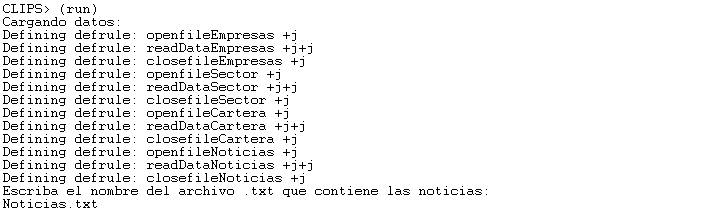
\includegraphics[width=25cm]{1.png} 
	\caption{Sistema Experto pide noticias.}
	\label{uno} 
\end{figure}

\begin{figure}[H]
	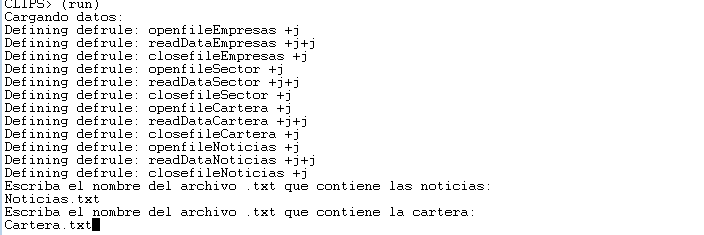
\includegraphics[width=25cm]{2.png} 
	\caption{Sistema Experto pide cartera del usuario.}
	\label{dos} 
\end{figure}

\begin{figure}[H]
	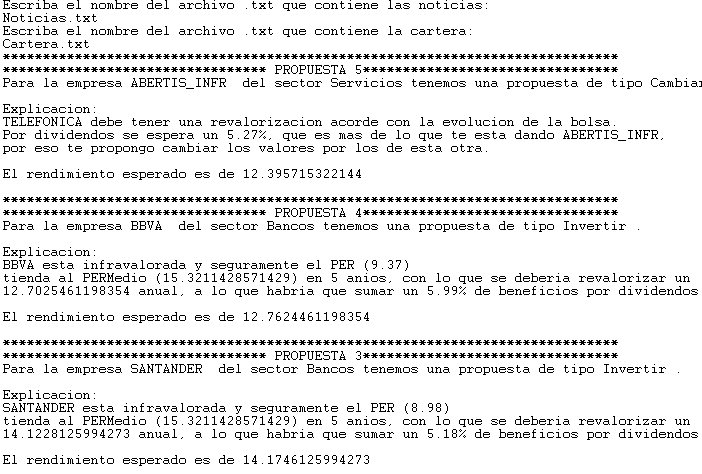
\includegraphics[width=15cm]{3.png} 
	\caption{Sistema Experto hace 5 mejores propuestas.}
	\label{tres} 
\end{figure}

\begin{figure}[H]
	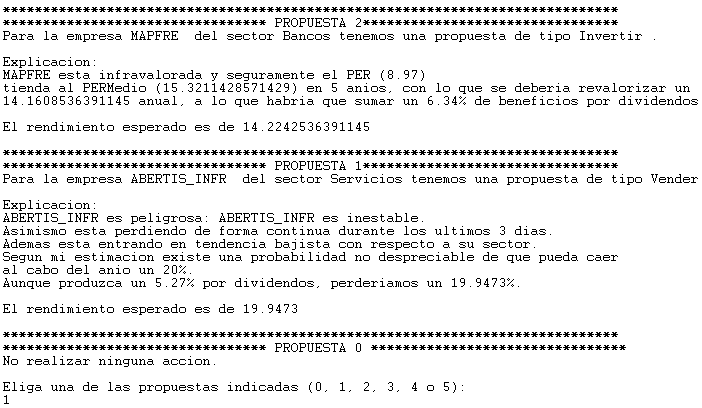
\includegraphics[width=15cm]{4.png} 
	\caption{Sistema Experto hace 5 mejores propuestas.}
	\label{cuatro} 
\end{figure}

\begin{figure}[H]
	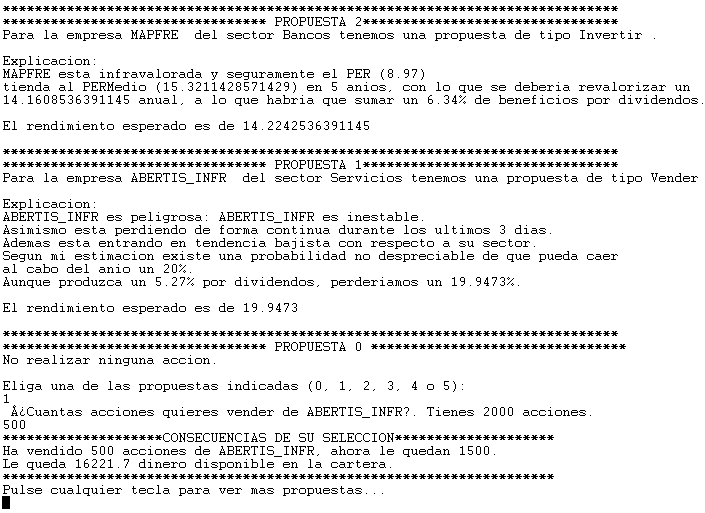
\includegraphics[width=18cm]{5.png} 
	\caption{Resultado de la elección.}
	\label{cinco} 
\end{figure}

\begin{figure}[H]
	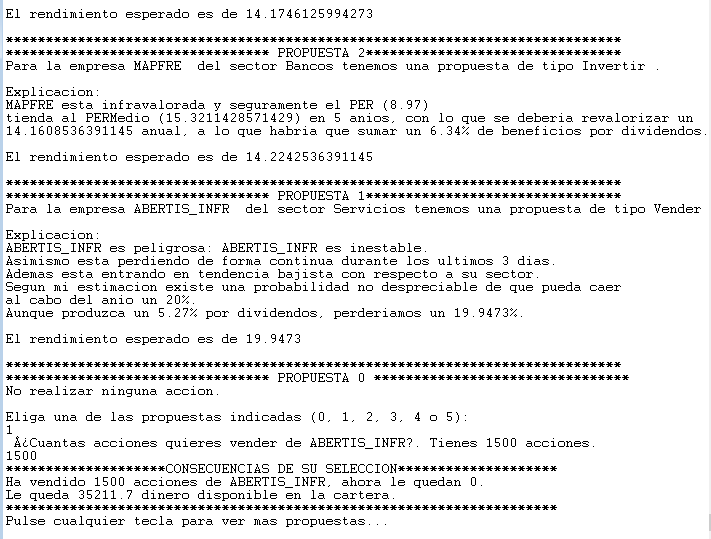
\includegraphics[width=18cm]{6.png} 
	\caption{Volvemos a vender acciones.}
	\label{seis} 
\end{figure}

\begin{figure}[H]
	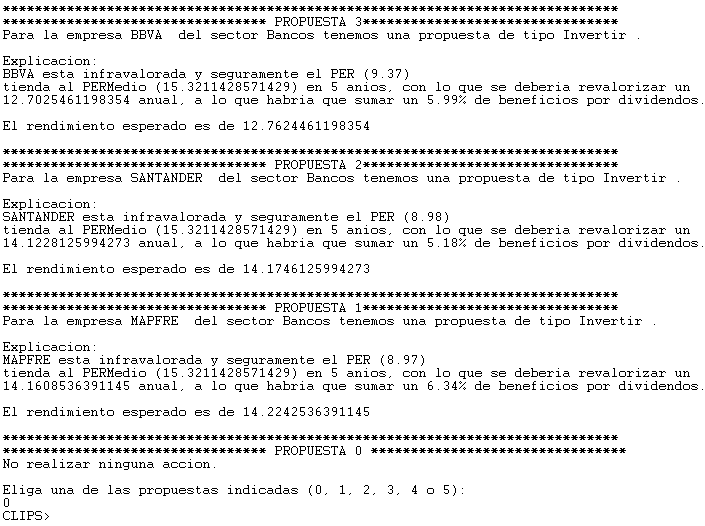
\includegraphics[width=18cm]{7.png} 
	\caption{Finalizo consulta.}
	\label{siete} 
\end{figure}


\end{document}
